\begin{frame}[fragile]{The expansion constant $\cexp$ is a type of dimension}

The \textbf{expansion constant} is defined as:
$$
\cexp = \sup_{p\in X, r\ge0} \left(
    \frac{|B(p,2r)|}{|B(p,r)|}
      \right)
$$
where
$$
B(p,r) = \{q \in X : d(p,q) \le r \}
$$
is the ball of radius $r$ centered at point $p$.
\vspace{0.15in}

\hrule
\vspace{0.15in}

%%%%%%%%%%%%%%%%%%%%%%%%%%%%%%%%%%%%%%%%

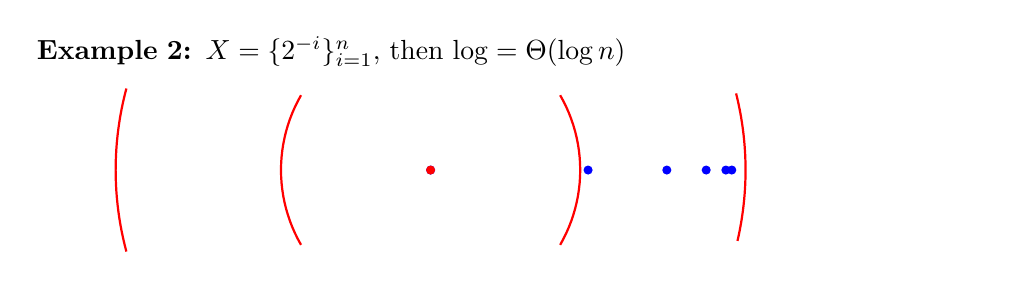
\begin{tikzpicture}

    %\node[text width=12cm] at (3,0) {\textbf{Example 1:} $X =$ regularly spaced points in $\R^d$, $\log\cexp=\Theta(d)$};
    %\foreach \i in {1,...,20} {
    %\foreach \j in {1,...,13} {
        %\node[draw=blue,minimum size=0.5mm,inner sep=0pt,outer sep=0pt,shape=circle,fill=blue] at (0.2*\i,-0.2*\j-0.3) {};
    %}}
%
    %\path[draw=red,fill=red]   (2,-1.7) circle (0.05);
    %\path[draw=red,very thick] (2,-1.7) circle (0.5);
    %\path[draw=red,very thick] (2,-1.7) circle (1);

    \node[text width=12cm] at (3,0) {\textbf{Example 2:} $X = \{ 2^{-i} \}_{i=1}^n$, then $\log\cexp = \Theta(\log n)$ };
    
    %\node[draw=blue,minimum size=0.5mm,inner sep=0pt,outer sep=0pt,shape=circle,fill=blue] at (-2,-1.5) {};
    \node[draw=blue,minimum size=1mm,inner sep=0pt,outer sep=0pt,shape=circle,fill=blue] at (2,-1.5) {};
    \node[draw=blue,minimum size=1mm,inner sep=0pt,outer sep=0pt,shape=circle,fill=blue] at (4,-1.5) {};
    \node[draw=blue,minimum size=1mm,inner sep=0pt,outer sep=0pt,shape=circle,fill=blue] at (5,-1.5) {};
    \node[draw=blue,minimum size=1mm,inner sep=0pt,outer sep=0pt,shape=circle,fill=blue] at (5.5,-1.5) {};
    \node[draw=blue,minimum size=1mm,inner sep=0pt,outer sep=0pt,shape=circle,fill=blue] at (5.75,-1.5) {};
    \node[draw=blue,minimum size=1mm,inner sep=0pt,outer sep=0pt,shape=circle,fill=blue] at (5.825,-1.5) {};

    \path[draw=red,fill=red]   (2,-1.5) circle (0.05);
    
    \draw [red,thick,domain=-150:-210] plot ({2+1.9*cos(\x)}, {-1.5+1.9*sin(\x)});
    \draw [red,thick,domain=-30:30] plot ({2+1.9*cos(\x)}, {-1.5+1.9*sin(\x)});

    \draw [red,thick,domain=-015:015] plot ({2+4.0*cos(\x)}, {-1.5+4.0*sin(\x)});
    \draw [red,thick,domain=-165:-195] plot ({2+4.0*cos(\x)}, {-1.5+4.0*sin(\x)});
    %\draw [red,thick,domain=-15:15] plot ({-2+3.9*cos(\x)}, {-1.5+3.9*sin(\x)});
    %\draw [red,thick,domain=-7.5:7.5] plot ({-2+8.0*cos(\x)}, {-1.5+8.0*sin(\x)});
\end{tikzpicture}

\end{frame}

